\documentclass{beamer}
\usetheme{CambridgeUS}
\usepackage[utf8]{inputenc}
\usepackage{graphicx}
\usepackage{amsmath}
\usepackage{mathrsfs}
\usepackage{stfloats}
\usepackage{bm}
\usepackage{cite}
\usepackage{cases}
\usepackage{subfig}
\usepackage{amsfonts}
\usepackage{amssymb}
\usepackage{mathtools}
\usepackage{tikz}
\usepackage{circuitikz}
\usepackage{verbatim}
\usepackage{calc}
\usepackage{float}
\usepackage{longtable}
\usepackage{multirow}
\usepackage{multicol}
\usepackage{color}
\usepackage{array}
\usepackage{hhline}
\usepackage{ifthen}
\usepackage{chngcntr}
\usepackage{hyperref}

\newcommand{\BEQA}{\begin{eqnarray}}
\newcommand{\EEQA}{\end{eqnarray}}
\newcommand{\define}{\stackrel{\triangle}{=}}
\def\inputGnumericTable{}

\let\vec\mathbf

\providecommand{\pr}[1]{\ensuremath{\Pr\left(#1\right)}}
\providecommand{\sbrak}[1]{\ensuremath{{}\left[#1\right]}}
\providecommand{\lsbrak}[1]{\ensuremath{{}\left[#1\right.}}
\providecommand{\rsbrak}[1]{\ensuremath{{}\left.#1\right]}}
\providecommand{\brak}[1]{\ensuremath{\left(#1\right)}}
\providecommand{\lbrak}[1]{\ensuremath{\left(#1\right.}}
\providecommand{\rbrak}[1]{\ensuremath{\left.#1\right)}}
\providecommand{\cbrak}[1]{\ensuremath{\left\{#1\right\}}}
\providecommand{\lcbrak}[1]{\ensuremath{\left\{#1\right.}}
\providecommand{\rcbrak}[1]{\ensuremath{\left.#1\right\}}}
\providecommand{\abs}[1]{\left\vert#1\right\vert}
\providecommand{\res}[1]{\Res\displaylimits_{#1}}
\newcommand{\myvec}[1]{\ensuremath{\begin{pmatrix}#1\end{pmatrix}}}
\newcommand{\mydet}[1]{\ensuremath{\begin{vmatrix}#1\end{vmatrix}}}

\title{AI1110: Probability and Random Variables}
\subtitle{Assignment 8}
\author{Vishal Vijay Devadiga (CS21BTECH11061)}
\date{\today}
\begin{document}

% Title page frame
\begin{frame}
    \titlepage
\end{frame}

% Remove logo from the next slides
\logo{}

% Outline frame
\begin{frame}{Outline}
    \tableofcontents
\end{frame}

% Beginning of Actual Doc
\section{Question}
\begin{frame}{Question}
    A fair die is rolled five times. Find the probability that one shows twice. three shows twice, and six shows once.
\end{frame}

\section{Solution}
\subsection{Theory}
\begin{frame}{Theory}
        For a Bernoulli trial, with events $A_1,A_2, \dots A_r$, and $\pr{A_i} = p_i$ where $\sum^r_{i=1} p_i = 1$, \\ 
        If the experiment is repeated n times where we denote by $p_n\brak{k_l,k_2,\dots,k_r}$, the probability of
        the event $A_i$ occurs $k_i$ times in any order where $\sum^r_{i=1} k_i = n$, then
        \begin{align}
            \label{eq:theory}
            p_n\brak{k_l,k_2,\dots,k_r} = \dfrac{n!}{k_1! k_2! \dots k_r!} p_1^{k_1} p_2^{k_2} \dots p_r^{k_r}
        \end{align}
\end{frame}

\subsection{PMF}
\begin{frame}{PMF}
    Let the random variable $X$ denote the number that appears on rolling the die. The PMF is given by:
    \begin{equation}
        \pr{X = k} = 
        \begin{cases}
            \dfrac{1}{6}, & 1 \geq k \geq 6 \\
            0, & \text{otherwise}
        \end{cases}
        \label{pmf}
    \end{equation}
    \begin{figure}[H]
        \centering
        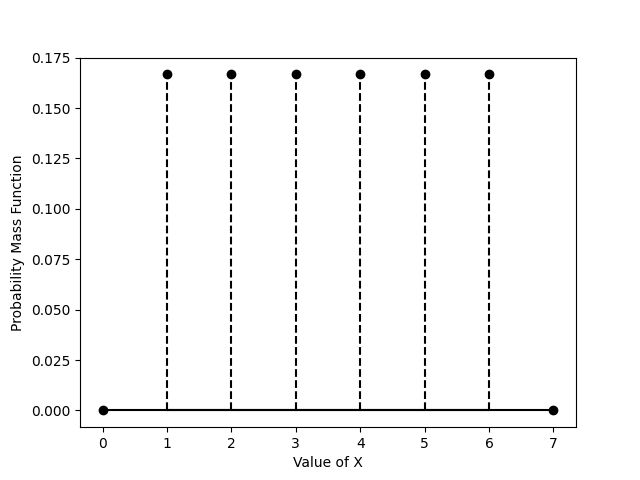
\includegraphics[scale = 0.39]{./figs/figure.png}
        \caption{}
        \label{fig:pmf}
    \end{figure}
\end{frame}

\subsection{Result}
\begin{frame}{Result}
    By \eqref{eq:theory} and \eqref{pmf},
    \begin{align}
        p_5\brak{2,0,2,0,0,1} &= \dfrac{5!}{2! 2! 1!} \brak{\frac{1}{6}}^2 \brak{\frac{1}{6}}^2 \brak{\frac{1}{6}}^1
        \\
        &= \dfrac{120}{4} \brak{\frac{1}{6}}^5
        \\
        \label{eq:result}
        &= \dfrac{5}{6^4}
    \end{align}
    By \eqref{eq:result}, the probability that one shows twice. three shows twice, and six shows once is $\dfrac{5}{6^4}$.
\end{frame}
\end{document}